\hypertarget{ux7b2cux4e00ux4e2a-python-ux7a0bux5e8f}{%
\subsection{第一个 Python
程序}\label{ux7b2cux4e00ux4e2a-python-ux7a0bux5e8f}}

在正式编写第一个 Python 程序前,我们先复习一下什么是命令行模式和 Python
交互模式。

\hypertarget{ux547dux4ee4ux884cux6a21ux5f0f}{%
\subsubsection{命令行模式}\label{ux547dux4ee4ux884cux6a21ux5f0f}}

在 Windows 开始菜单选择
``命令提示符'',就进入到命令行模式,它的提示符类似\texttt{C:\textbackslash{}\textgreater{}}:

\begin{pythoncode}
┌────────────────────────────────────────────────────────┐
│Command Prompt                                    - □ x │
├────────────────────────────────────────────────────────┤
│Microsoft Windows [Version 10.0.0]                      │
│(c) 2015 Microsoft Corporation. All rights reserved.    │
│                                                        │
│C:\> _                                                  │
│                                                        │
│                                                        │
│                                                        │
│                                                        │
│                                                        │
│                                                        │
│                                                        │
└────────────────────────────────────────────────────────┘
\end{pythoncode}

\hypertarget{python-ux4ea4ux4e92ux6a21ux5f0f}{%
\subsubsection{Python 交互模式}\label{python-ux4ea4ux4e92ux6a21ux5f0f}}

在命令行模式下敲命令\texttt{python},就看到类似如下的一堆文本输出,然后就进入到
Python
交互模式,它的提示符是\texttt{\textgreater{}\textgreater{}\textgreater{}}。

\begin{pythoncode}
┌────────────────────────────────────────────────────────┐
│Command Prompt - python                           - □ x │
├────────────────────────────────────────────────────────┤
│Microsoft Windows [Version 10.0.0]                      │
│(c) 2015 Microsoft Corporation. All rights reserved.    │
│                                                        │
│C:\> python                                             │
│Python 3.7 ... on win32                                 │
│Type "help", ... for more information.                  │
│>>> _                                                   │
│                                                        │
│                                                        │
│                                                        │
│                                                        │
└────────────────────────────────────────────────────────┘
\end{pythoncode}

在 Python 交互模式下输入\texttt{exit()}并回车,就退出了 Python
交互模式,并回到命令行模式:

\begin{pythoncode}
┌────────────────────────────────────────────────────────┐
│Command Prompt                                    - □ x │
├────────────────────────────────────────────────────────┤
│Microsoft Windows [Version 10.0.0]                      │
│(c) 2015 Microsoft Corporation. All rights reserved.    │
│                                                        │
│C:\> python                                             │
│Python 3.7 ... on win32                                 │
│Type "help", ... for more information.                  │
│>>> exit()                                              │
│                                                        │
│C:\> _                                                  │
│                                                        │
│                                                        │
└────────────────────────────────────────────────────────┘
\end{pythoncode}

也可以直接通过开始菜单选择\texttt{Python\ (command\ line)}菜单项,\emph{直接进入}
Python
交互模式,但是输入\texttt{exit()}后窗口会直接关闭,不会回到命令行模式。

了解了如何启动和退出 Python 的交互模式,我们就可以正式开始编写 Python
代码了。

在写代码之前,请\_千万不要\_用 ``复制''-``粘贴''
把代码从页面粘贴到你自己的电脑上。写程序也讲究一个感觉,你需要一个字母一个字母地把代码自己敲进去,在敲代码的过程中,初学者经常会敲错代码:拼写不对,大小写不对,混用中英文标点,混用空格和
Tab 键,所以,你需要仔细地检查、对照,才能以最快的速度掌握如何写程序。

 
 \begin{figure}[htp]
	\centering
	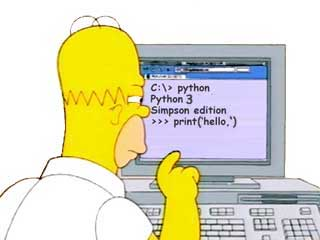
\includegraphics[width=0.6\linewidth]{fig/1017024373322432l.png}
\end{figure}


在交互模式的提示符\texttt{\textgreater{}\textgreater{}\textgreater{}}下,直接输入代码,按回车,就可以立刻得到代码执行结果。现在,试试输入\texttt{100+200},看看计算结果是不是
300:

\begin{pythoncode}
>>> 100+200
300
\end{pythoncode}

很简单吧,任何有效的数学计算都可以算出来。

如果要让 Python
打印出指定的文字,可以用\texttt{print()}函数,然后把希望打印的文字用单引号或者双引号括起来,但不能混用单引号和双引号:

\begin{pythoncode}
>>> print('hello, world')
hello, world
\end{pythoncode}

这种用单引号或者双引号括起来的文本在程序中叫字符串,今后我们还会经常遇到。

最后,用\texttt{exit()}退出 Python,我们的第一个 Python
程序完成!唯一的缺憾是没有保存下来,下次运行时还要再输入一遍代码。

\hypertarget{ux547dux4ee4ux884cux6a21ux5f0fux548c-python-ux4ea4ux4e92ux6a21ux5f0f}{%
\subsubsection{命令行模式和 Python
交互模式}\label{ux547dux4ee4ux884cux6a21ux5f0fux548c-python-ux4ea4ux4e92ux6a21ux5f0f}}

请注意区分命令行模式和 Python 交互模式。

在命令行模式下,可以执行\texttt{python}进入 Python
交互式环境,也可以执行\texttt{python\ hello.py}运行一个\texttt{.py}文件。

执行一个\texttt{.py}文件\_只能\_在命令行模式执行。如果敲一个命令\texttt{python\ hello.py},看到如下错误:

\begin{pythoncode}
┌────────────────────────────────────────────────────────┐
│Command Prompt                                    _ □ x │
├────────────────────────────────────────────────────────┤
│Microsoft Windows [Version 10.0.0]                      │
│(c) 2015 Microsoft Corporation. All rights reserved.    │
│                                                        │
│C:\> python hello.py                                    │
│python: can't open file 'hello.py': [Errno 2] No such   │
│file or directory                                       │
│                                                        │
│                                                        │
│                                                        │
│                                                        │
│                                                        │
└────────────────────────────────────────────────────────┘
\end{pythoncode}

错误提示\texttt{No\ such\ file\ or\ directory}说明这个\texttt{hello.py}在当前目录\_找不到\_,必须先把当前目录切换到\texttt{hello.py}所在的目录下,才能正常执行:

\begin{pythoncode}
┌────────────────────────────────────────────────────────┐
│Command Prompt                                    _ □ x │
├────────────────────────────────────────────────────────┤
│Microsoft Windows [Version 10.0.0]                      │
│(c) 2015 Microsoft Corporation. All rights reserved.    │
│                                                        │
│C:\> cd work                                            │
│                                                        │
│C:\work> python hello.py                                │
│Hello, world!                                           │
│                                                        │
│                                                        │
│                                                        │
│                                                        │
└────────────────────────────────────────────────────────┘
\end{pythoncode}

此外,在命令行模式运行\texttt{.py}文件和在 Python 交互式环境下直接运行
Python 代码有所不同。Python 交互式环境会把每一行 Python
代码的结果自动打印出来,但是,直接运行 Python 代码却不会。

例如,在 Python 交互式环境下,输入:

\begin{pythoncode}
>>> 100 + 200 + 300
600
\end{pythoncode}

直接可以看到结果\texttt{600}。

但是,写一个\texttt{calc.py}的文件,内容如下:

\begin{pythoncode}
100 + 200 + 300
\end{pythoncode}

然后在命令行模式下执行:

\begin{pythoncode}
C:\work>python calc.py
\end{pythoncode}

发现什么输出都没有。

这是正常的。想要输出结果,必须自己用\texttt{print()}打印出来。把\texttt{calc.py}改造一下:

\begin{pythoncode}
print(100 + 200 + 300)
\end{pythoncode}

再执行,就可以看到结果:

\begin{pythoncode}
C:\work>python calc.py
600
\end{pythoncode}

最后,Python
交互模式的代码是输入一行,执行一行,而命令行模式下直接运行\texttt{.py}文件是一次性执行该文件内的所有代码。可见,Python
交互模式主要是为了调试 Python
代码用的,也便于初学者学习,它\_不是\_正式运行 Python 代码的环境!

\hypertarget{ux5c0fux7ed3}{%
\subsubsection{小结}\label{ux5c0fux7ed3}}

在 Python 交互式模式下,可以直接输入代码,然后执行,并立刻得到结果。

在命令行模式下,可以直接运行\texttt{.py}文件。

